\chapter[Introdução]{Introdução}

Dentre os acidentes automotivos, os que possuem o maior número de vítimas fatais
são do tipo colisão frontal.
De 2010 a 2014 quase metade dos acidentes com
fatalidades em rodovias federais, um total de 48,3\%, foram fruto desse tipo de colisão e de
atropelamentos. É um tipo de acidente que embora possua baixa ocorrência é extremamente violento. \cite{ipea}

	Ao contrário do que se pensa, a maioria dos acidentes ocorre a luz do dia, com tempo bom.
  De acordo com a Polícia Rodoviária Federal os motoristas envolvidos em acidentes não estão
  cansados, dirigem no máximo uma hora, sendo a imprudência causa
  principal de acidentes. \cite{acidentesDeTransitoNoBrasil}

	Essas informações recebem comprovação nos relatórios do IPEA, de 2008, informando que colisões
   frontais representam 4\% de todos os acidentes embora possua uma parcela 24,6\% do total de
   mortes. 81,75\% dos acidentes desse tipo ocorreram em pistas simples com tráfego nos dois
   sentidos e o principal motivo apontado seriam: ultrapassagem indevida, ultrapassagem de
   veículos lentos ou em congestionamento e falta de visibilidade. \cite{fatoresCondicionantesGravidade}

	Em outro relatório do IPEA, de 2004, curiosamente mantém a mesma porcentagem apresentada no
   relatório recente de 2008 e pode ser acompanhado na Figura \ref{fig:introducao}. \cite{custos_acidentes_transito}

   \begin{figure}[h]
     \centering
     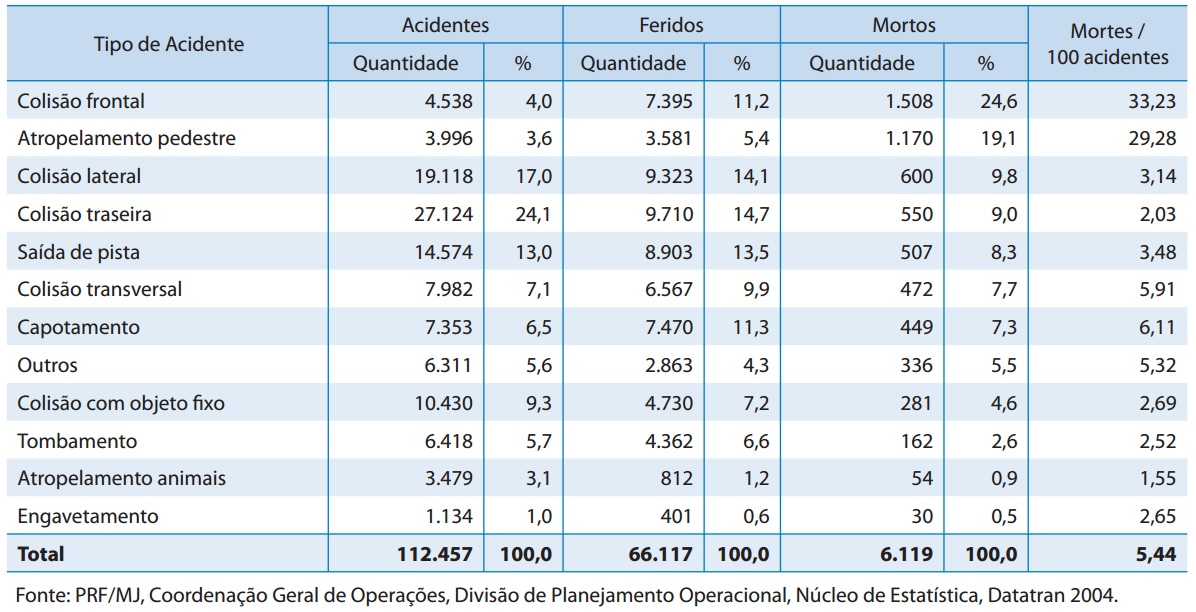
\includegraphics[width=450px, scale=0.5]{figuras/introducao}
     \caption{Tipo versus Gravidade dos acidentes em rodovias federais – 2004}
     \label{fig:introducao}
   \end{figure}


   Mediante análise dos dados apontados foi identificada uma demanda e este relatório
   contempla o desenvolvimento de um projeto preliminar para um sistema que auxilie o
   condutor a realizar ultrapassagens em rodovias simples, de mão dupla, com segurança,
	a fim de evitar que motoristas tomem a decisão de fazer manobras arriscadas
	de ultrapassagem, baseados apenas na própria experiência ou no bom senso.

	Com o auxílio dos sensores LIDAR e Radar para detectar a distância de outros
	veículos; sensores de rotação , o indicador da seta do veículo e a câmara
	capaz de detectar mudanças de faixa, para identificar intenção de ultrapassagem;
	um sistema de comunicação que utiliza da tecnologia dos transponders; Um GPS
	para auxiliar na identificação da posição do veículo, o sistema emitirá alertas
	de colisão indicando quando é seguro ultrapassar um veículo. Este conjunto
	de equipamentos, juntamente com os controladores/processadores detectarão os
	veículos ao redor, realizarão os cálculos em tempo real para determina as
	distâncias e velocidades, além da direção e sentido deles, a fim de auxiliar
	o condutor na tomada de decisão da ultrapassagem ou alertá-lo caso esta não
	seja viável.

	Desta forma, este sistema não tem como objetivo atuar sobre os comandos do
	 veículo. Será de sua responsabilidade apenas informar ao usuário se é
	segura ou não uma manobra.

Espera-se que o projeto deste sistema seja capaz de auxiliar na construção e
comercialização desta tecnologia de prevenção de acidentes e que todos os
veículos contenham-na, a fim de que ela reduza os índices de colisões
frontais nas rodovias brasileiras.
